\documentclass{article}

\usepackage[utf8x]{inputenc}
\usepackage[english]{babel}
\usepackage{hyperref}

\usepackage{amsmath,amsfonts,amsthm,amssymb,enumerate,fullpage,tikz}
\setlength{\parindent}{0pt}
\usepackage{listings}
\usepackage{color}
\newcommand{\mb}[1]{\mathbb{#1}}
\newcommand{\mc}[1]{\mathcal{#1}}
\newcommand{\Z}{\mb{Z}}
\newcommand{\N}{\mb{N}}
\newcommand{\R}{\mb{R}}
\newcommand{\C}{\mb{C}}
\newcommand{\cproj}{\C\textup{P}^\infty}
\DeclareMathOperator{\myker}{ker}
\DeclareMathOperator{\im}{im}
\DeclareMathOperator{\Tor}{Tor}
\usetikzlibrary{arrows}


%% Theorem environment declarations (using amsthm):
\newtheorem{theorem}{Theorem}[section]
\newtheorem{axiom}[theorem]{Axiom}
\newtheorem{fact}[theorem]{Fact}
\newtheorem{proposition}[theorem]{Proposition}
\newtheorem{lemma}[theorem]{Lemma}
\newtheorem{corollary}[theorem]{Corollary}

\theoremstyle{definition}
\newtheorem{definition}[theorem]{Definition}
\newtheorem{convention}[theorem]{Convention}
\newtheorem{examplex}[theorem]{Example}
\newenvironment{example}
  {\pushQED{\qed}\renewcommand{\qedsymbol}{$\triangle$}\examplex}
  {\popQED\endexamplex}
\newtheorem{examples}[theorem]{Examples}
\newtheorem{notation}[theorem]{Notation}
\theoremstyle{remark}
\newtheorem{remark}[theorem]{Remark}
\newtheorem{idea}[theorem]{Idea}


\begin{document}

\title{Applications of the Serre Spectral Sequence}
\author{Floris van Doorn}
\date{November 10, 2015}
\maketitle

\section{Serre Spectral Sequence}

\begin{definition}
A \emph{Spectral Sequence} is a sequence $(E_{p,q}^r,d_r)$ consisting of
\begin{itemize}
\item An $R$-module $E^r_{p,q}$ for $p,q\in \Z$ and $r\geq 0$.
\item Differentials $d_{p,q}^r : E_{p,q}^r\to E_{p-r,q+r-1}^r$ such that $d_r^2=0$
\end{itemize}
where $E^{r+1}$ is defined to be the homology of $(E^r,d^r)$. That is,
$E_{p,q}^{r+1}=\myker(d_{p,q}^r)/\im(d_{p+r,q-r+1}^r)$. The variable $r$ is called the \emph{page}, $p$ the \emph{filtration degree}, $q$ the \emph{complementary degree} and $p+q$ the \emph{total degree}.
\end{definition}

\begin{theorem}[Serre Spectral Sequence]
Let $F \to X \twoheadrightarrow B$ be a fibration such that $B$ is path-connected and $\pi_1(B)$
acts trivially on $H_*(F;G)$. Then
$$H_p(B;H_q(F;G))\ \Longrightarrow\ H_{p+q}(X;G).$$ This means that there is a spectral sequence
$(E_{p,q}^r,d_r)$ where $E_{p,q}^2\simeq H_p(B;H_q(F;G))$ and there is a filtration $0 \subseteq
F_{p+q}^0 \subseteq \cdots \subseteq F_{p+q}^{p+q}=H_{p+q}(X;G)$ such that $E_{p,q}^\infty\simeq
F_{p+q}^p/F_{p+q}^{p-1}$.
\end{theorem}

Note that if $B$ is simply connected, then conditions of the theorem are satisfied.


\subsection{Examples}

\begin{example}
Suppose $X=B\times F$, where $B$ is path-connected, and suppose that $G$ is a field. Then $\pi_1(B)$
acts trivially on $H_*(F;G)$ and we have
\begin{align*}
H_n(X;G) &= \bigoplus_{p+q=n}H_p(B;G)\otimes H_q(F;G)&&\text{(K\"unneth formula)}\\
&=\bigoplus_{p+q=n}H_p(B;H_q(F;G))&&\text{(Univ. Coeff. Th. for homology)}\\
\end{align*}
This means that all entries in the second page survive until page infinity. The other extreme is if
$X$ is contractible, where almost nothing will survive, as we will see in the next examples.
\end{example}

In the next example, we will use that $S^1=K(\Z,1)$ and $\cproj=K(\Z,2)$.

\begin{example}
Consider the path space fibration of $B=\cproj$, that is $\Omega B\to PB \twoheadrightarrow B$ and
note that $S^1=\Omega B$. Since $B$ is simply connected, we can apply the Serre Spectral Sequence
with coefficients in $\Z$. We know that $E_{p,q}^2\simeq H_p(B;H_q(S^1))$ and $H_q(S^1)=0$ for $q>1$
and $\Z$ for $q=0,1$. This means that the page $E^2$ looks like this.

\begin{center}
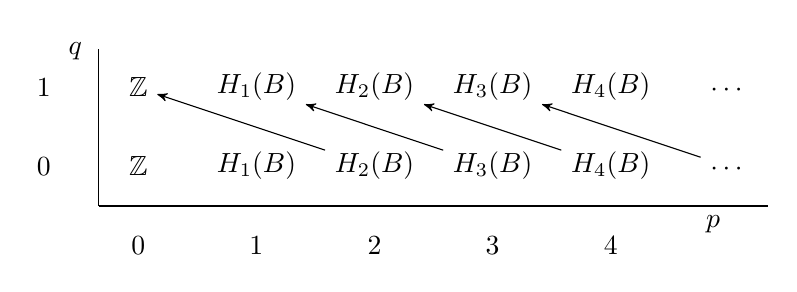
\begin{tikzpicture}[>=stealth',auto,node distance=1.5cm,
  main node/.style={font=\sffamily\bfseries},text height=1.5ex]
  \node[main node]   (-11)at (-1.2,0.8)   {\mbox{}};
  \node[main node]   (00) at (0,0)      {$\Z$};
  \node[main node]   (01) at (0,1)      {$\Z$};
  \node[main node]   (10) at (1.5,0)    {$H_1(B)$};
  \node[main node]   (11) at (1.5,1)    {$H_1(B)$};
  \node[main node]   (20) at (3,0)      {$H_2(B)$};
  \node[main node]   (21) at (3,1)      {$H_2(B)$};
  \node[main node]   (30) at (4.5,0)    {$H_3(B)$};
  \node[main node]   (31) at (4.5,1)    {$H_3(B)$};
  \node[main node]   (40) at (6,0)      {$H_4(B)$};
  \node[main node]   (41) at (6,1)      {$H_4(B)$};
  \node[main node]   (50) at (7.5,0)    {$\cdots$};
  \node[main node]   (51) at (7.5,1)    {$\cdots$};
  \node at (-1.2,1) {1};
  \node at (-1.2,0) {0};
  \node at (0,-1)   {0};
  \node at (1.5,-1) {1};
  \node at (3,-1)   {2};
  \node at (4.5,-1) {3};
  \node at (6,-1)   {4};
  \node at (7.3,-0.7)   {$p$};
  \node at (-0.8,1.5)   {$q$};
  \draw (-0.5,-0.5) -- (8,-0.5);
  \draw (-0.5,-0.5) -- (-0.5,1.5);
  \path[every node/.style={font=\sffamily\small}]
%    (10) edge [->] (-11)
    (20) edge [->] (01)
    (30) edge [->] (11)
    (40) edge [->] (21)
    (50) edge [->] (31);
\end{tikzpicture}
\end{center}

Moreover, we have $E_{p,q}^\infty=\Z$ for $p=q=0$ and $0$ otherwise. From this we can conclude that
$$H_i(\cproj,\Z)=\begin{cases} \Z & \text{if $i$ even} \\ 0 & \text{if $i$ odd.}\end{cases}$$
\end{example}

\begin{example}
In this example we will compute the homology groups of the loop space of the sphere, $\Omega S^n$
for $n\geq 2$. We use the fibration $\Omega S^n \to PS^n \twoheadrightarrow S^n$ and we can apply the Serre
Spectral Sequence, since $S^n$ is simply connected. Now $H_p(S^n;G)=G$ for $p=0,n$ and $0$
otherwise. This means that only the $0$ and the $n$ column can be nonzero.

\begin{center}
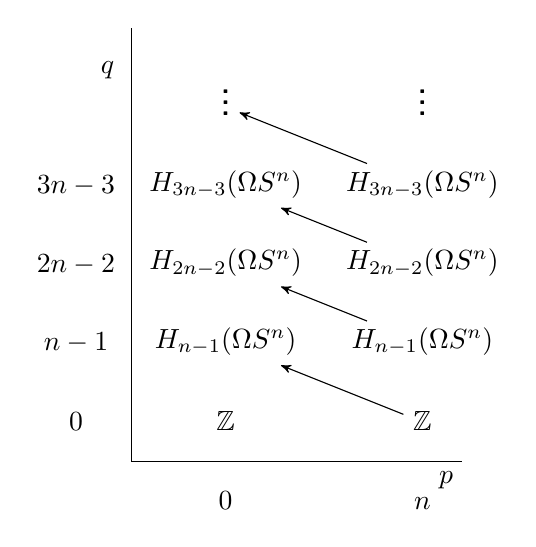
\begin{tikzpicture}[>=stealth',auto,node distance=1.5cm,
  main node/.style={font=\sffamily\bfseries},text height=1.5ex]
  \node[main node]   (00) at (0,0)      {$\Z$};
  \node[main node]   (10) at (2.5,0)    {$\Z$};
  \node[main node]   (01) at (0,1)      {$H_{n-1}(\Omega S^n)$};
  \node[main node]   (11) at (2.5,1)    {$H_{n-1}(\Omega S^n)$};
  \node[main node]   (02) at (0,2)      {$H_{2n-2}(\Omega S^n)$};
  \node[main node]   (12) at (2.5,2)    {$H_{2n-2}(\Omega S^n)$};
  \node[main node]   (03) at (0,3)      {$H_{3n-3}(\Omega S^n)$};
  \node[main node]   (13) at (2.5,3)    {$H_{3n-3}(\Omega S^n)$};
  \node[main node]   (04) at (0,4)      {$\vdots$};
  \node[main node]   (14) at (2.5,4)    {$\vdots$};
  \node at (-1.9,0) {0};
  \node at (-1.9,1) {$n-1$};
  \node at (-1.9,2) {$2n-2$};
  \node at (-1.9,3) {$3n-3$};
  \node at (0,-1)   {0};
  \node at (2.5,-1) {$n$};
  \node at (2.8,-0.7)   {$p$};
  \node at (-1.5,4.5)   {$q$};
  \draw (-1.2,-0.5) -- (3,-0.5);
  \draw (-1.2,-0.5) -- (-1.2,5);
  \path[every node/.style={font=\sffamily\small}]
    (10) edge [->] (01)
    (11) edge [->] (02)
    (12) edge [->] (03)
    (13) edge [->] (04);
\end{tikzpicture}
\end{center}
After some reasoning, we get that $H_i(\Omega S^n,\Z)=\begin{cases} \Z & \text{for $n-1\mid i$}\\ 0 & \text{otherwise.}\end{cases}$
\end{example}


\section{Serre Class Theorem}

\begin{definition}
We say that a space $X$ is \emph{abelian} if the action of $\pi_1(X)$ on $\pi_n(X)$ is trivial for all $n\geq 1$.
\end{definition}
Note that every simply connected space is abelian.
\begin{definition}
  A \emph{Serre Class} is a class $\mc C$ of abelian groups containing the trivial group such that for every SES $0\to A\to B\to C\to 0$ we have $B\in\mc C$ iff $A,C\in \mc C$. In this document I call a Serre class \emph{nice} if for every $A,B\in\mc C$ also $A\otimes B$ and $\Tor(A,B)$ are in $\mc C$. (this name is made up by me)
\end{definition}
\begin{lemma}
  The following classes are nice Serre classes.
\begin{itemize}
\item $\mc {FG}$, the class of finitely generated abelian groups
\item $\mc{T}_P$ for some set $P$ of primes. This is the class of torsion abelian groups whose
  elements have orders divisible only by primes in $P$.
\item $\mc{F}_P$, the finite groups in $\mc{T}_P$.
\end{itemize}
\end{lemma}
Note that $P$ is the set of all primes $\mc{T}_P$ becomes the class of all torsion abelian groups
and $\mc{F}_P$ becomes the class of all finite abelian groups.

\begin{theorem}
  Let $X$ be a path-connected and abelian space, and let $\mc C$ be a nice Serre class. Then
  $$\forall(n>0)(\pi_n(X)\in\mc{C})\quad \longleftrightarrow\quad \forall(n>0)(H_n(X)\in\mc{C})$$
\end{theorem}

\begin{corollary}
The homotopy groups of a finite simply connected CW-complex are finitely generated. In particular, the homotopy groups of spheres are finitely generated.
\end{corollary}

Recall the following definition and theorem.
\begin{definition}
The \emph{Hurewicz homomorphism} is the homomorphism $h : \pi_n(X) \to H_n(X)$ defined by $h([f])=f_*(\gamma)$, where $\gamma$ is a generator of $H_n(S^n)\simeq\Z$.
\end{definition}

\begin{theorem}[Hurewicz]
Let $n\geq2$ and $X$ a $(n-1)$-connected space. Then $\widetilde H_i(X)=0$ for $i<n$ and the Hurewicz homomorphism $h : \pi_n(X) \to H_n(X)$ is an isomorphism.
\end{theorem}

We will now generalize this theorem.
\begin{theorem}
  Let $X$ be a path-connected and abelian space, and let $\mc C$ be a nice Serre class. Suppose that $\pi_i(X)\in\mc C$ for $i<n$. Then the Hurewicz homomorphism $h:\pi_n(X)\to H_n(X)$ is an isomorphism modulo $\mc{C}$, which means that its kernel and cokernel are in $\mc{C}$.
\end{theorem}

\section{Cohomology Serre Spectral Sequence}

There is a Serre Spectral Sequence for cohomology which is completely analogous. Of course, the
arrows in these spectral sequences are reversed.

\begin{theorem}
Let $F \to X \twoheadrightarrow B$ be a fibration such that $B$ is path-connected and $\pi_1(B)$
acts trivially on $H_*(F;G)$. Then
$$H^p(B;H^q(F;G))\ \Longrightarrow\ H^{p+q}(X;G).$$
\end{theorem}

However, we can now also use the cup product if the underlying group is a ring.

\begin{theorem}
  There is a bilinear product $E_r^{p,q}\times E_r^{s,t}\to E_r^{p+s,q+t}$ for $1\leq r\leq \infty$
  (written as concatenation) satisfying
  \begin{itemize}
  \item For $x\in E^{p,q}_r$ we define $|x|=p+q$. Then we have
    $d_r(xy)=(d_rx)y+(-1)^{|x|}x(d_ry)$. This means that the product on level $r$ induces a product
    on level $r+1$, which coincides with the given bilinear product at level $r+1$. The product in
    $E_\infty$ is induces from the products at the finite levels.
  \item At page 2, the product is up to a factor $(-1)^{qs}$ induced from the cup product under the
    correspondence $E_2^{p,q}\simeq H^p(B;H^q(F;R))$. In the RHS the cup product sends $(\phi,\psi)$
    to $\phi\smallsmile\psi$ and coefficients are also multiplied via the cup product.
  \item The cup product in $H^*(X;R)$ restricts to maps on the filtrations $F_p^m\times F_s^n\to
    F_{p+s}^{m+n}$ which induce quotient maps $F_p^m/F_{p+1}^m\times F_s^n/F_{s+1}^n\to
    F_{p+s}^{m+n}/F_{p+s+1}^{m+n}$. Under the correspondence $E^{p,q}_\infty\simeq
    F^{p+q}_p/F^{p+q}_{p+1}$ the product in the LHS corresponds to these maps in the RHS.
  \item $ab=(-1)^{|a||b|}ba$ and $d(x^n)=nx^{n-1}dx$ if $|x|$ is even.
  \end{itemize}
\end{theorem}

In particular, if we apply the cup $E_2^{p,0}\times E_2^{0,q}\to E_2^{p,q}$ to a pair of units, we
get a unit.

\subsection{Examples}

\begin{example}
Consider the path space fibration of $B=\cproj$ again. By the universal coefficient theorem, we know
that the cohomology groups are the same as the homology groups. Now let's compute the cup product
structure. Let $x_{2i}$ be the generator of $E_2^{2i,0}$ and $a$ the generator of $E_2^{0,1}$. Then
$x_0$ is the unit for multiplication, and $ax_{2i}$ are generators of $E_2^{2i,1}$.
\begin{center}
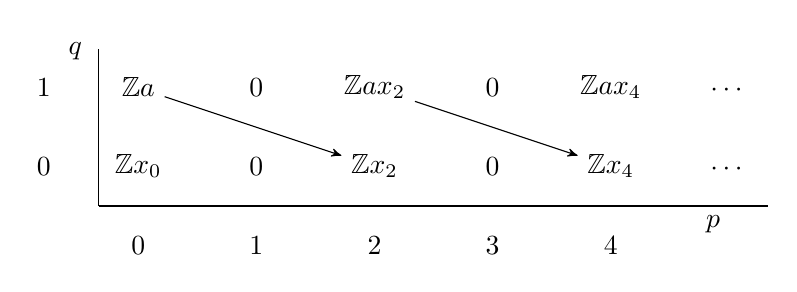
\begin{tikzpicture}[>=stealth',auto,node distance=1.5cm,
  main node/.style={font=\sffamily\bfseries},text height=1.5ex]
  \node[main node]   (-11)at (-1.2,0.8)   {\mbox{}};
  \node[main node]   (00) at (0,0)      {$\Z x_0$};
  \node[main node]   (01) at (0,1)      {$\Z a$};
  \node[main node]   (10) at (1.5,0)    {$0$};
  \node[main node]   (11) at (1.5,1)    {$0$};
  \node[main node]   (20) at (3,0)      {$\Z x_2$};
  \node[main node]   (21) at (3,1)      {$\Z ax_2$};
  \node[main node]   (30) at (4.5,0)    {$0$};
  \node[main node]   (31) at (4.5,1)    {$0$};
  \node[main node]   (40) at (6,0)      {$\Z x_4$};
  \node[main node]   (41) at (6,1)      {$\Z ax_4$};
  \node[main node]   (50) at (7.5,0)    {$\cdots$};
  \node[main node]   (51) at (7.5,1)    {$\cdots$};
  \node at (-1.2,1) {1};
  \node at (-1.2,0) {0};
  \node at (0,-1)   {0};
  \node at (1.5,-1) {1};
  \node at (3,-1)   {2};
  \node at (4.5,-1) {3};
  \node at (6,-1)   {4};
  \node at (7.3,-0.7)   {$p$};
  \node at (-0.8,1.5)   {$q$};
  \draw (-0.5,-0.5) -- (8,-0.5);
  \draw (-0.5,-0.5) -- (-0.5,1.5);
  \path[every node/.style={font=\sffamily\small}]
%    (10) edge [->] (-11)
    (01) edge [->] (20)
    (21) edge [->] (40);
\end{tikzpicture}
\end{center}
All arrows are isomorphisms. We may assume that $d_2a=x_2$. Then we compute $d_2(ax_{2i})=x_2x_{2i}$ so we may assume that $x_2x_{2i}=x_{2i+2}$. This gives $x_{2i}=x_2^i$. Hence $H^*(\cproj,\Z)\simeq \Z[x_2]$.
\end{example}

\begin{example}
We will compute the cup product structure of $H^*(\Omega S^n;\Z)$ using the path space fibration of $S^n$ for $n\geq2$. The additive structure is the same as for homology, and we can name the generators as in the figure, where $a_0=1$.
\begin{center}
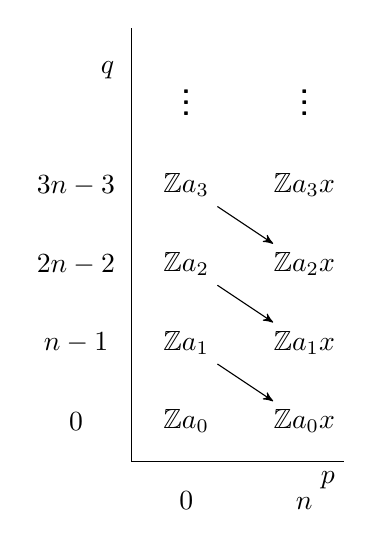
\begin{tikzpicture}[>=stealth',auto,node distance=1.5cm,
  main node/.style={font=\sffamily\bfseries},text height=1.5ex]
  \node[main node]   (00) at (0,0)      {$\Z a_0$};
  \node[main node]   (10) at (1.5,0)    {$\Z a_0x$};
  \node[main node]   (01) at (0,1)      {$\Z a_1$};
  \node[main node]   (11) at (1.5,1)    {$\Z a_1x$};
  \node[main node]   (02) at (0,2)      {$\Z a_2$};
  \node[main node]   (12) at (1.5,2)    {$\Z a_2x$};
  \node[main node]   (03) at (0,3)      {$\Z a_3$};
  \node[main node]   (13) at (1.5,3)    {$\Z a_3x$};
  \node[main node]   (04) at (0,4)      {$\vdots$};
  \node[main node]   (14) at (1.5,4)    {$\vdots$};
  \node at (-1.4,0) {0};
  \node at (-1.4,1) {$n-1$};
  \node at (-1.4,2) {$2n-2$};
  \node at (-1.4,3) {$3n-3$};
  \node at (0,-1)   {0};
  \node at (1.5,-1) {$n$};
  \node at (1.8,-0.7)   {$p$};
  \node at (-1,4.5)   {$q$};
  \draw (-0.7,-0.5) -- (2,-0.5);
  \draw (-0.7,-0.5) -- (-0.7,5);
  \path[every node/.style={font=\sffamily\small}]
    (01) edge [->] (10)
    (02) edge [->] (11)
    (03) edge [->] (12);
\end{tikzpicture}
\end{center}
We may assume that $d(a_{k+1})=a_kx$ and note that $a_kx=xa_k$.

We distinguish two cases.

\emph{If $n$ is odd} we compute by induction to $i+j$ that $a_ia_j={i+j \choose i}a_{i+j}$. Hence $H^*(\Omega S^n,\Z)\simeq \Gamma_{\Z}[a_1]$, where the \emph{divided polynomial algebra} $\Gamma_R[\alpha]$ is the quotient of the free $R$-algebra $R[\alpha_1,\alpha_2,\ldots]$ by the relations $\alpha_i\alpha_j={i+j \choose i}\alpha_{i+j}$.

\emph{If $n$ is even}, then we compute $a_1^2=0$ and by induction on $k$ we compute $a_1a_{2k}=a_{2k+1}$ and $a_1a_{2k+1}=0$ and $a_2^k=k!a_{2k}$.


Now $H^*(\Omega S^n,\Z)\simeq \Lambda_\Z[a_1]\otimes \Gamma_\Z[a_2]$ where the \emph{exterior algebra} $\Lambda_R[\alpha_1,\alpha_2,\ldots]$ is the free $R$-module with basis finite products $\alpha_{i_1}\cdots\alpha_{i_k}$ for $i_1<\cdots<i_k$ where multiplication is defined as $\alpha_i\alpha_j=-\alpha_j\alpha_i$ and $\alpha_i^2=0$.
\end{example}

For the next example, we use the following.

\begin{remark}
We can factor any map $f:A\to B$ as a homotopy equivalence followed by a fibration: $A \stackrel{\sim}{\to} E_f \to B$. Here $E_f=\{(a,\gamma)\in A\times B^I\mid \gamma(0)=f(a)\}$. In HoTT we would have $E_f=\Sigma(x:A)\Sigma(y:B), f(a) = y$.
\end{remark}
\begin{example}
In this example we will proof that the $p$-torsion subgroups of $\pi_i(S^3)$ is $0$ for $i<2p$ and $\Z_p$ for $i=2p$. Start with a map $S^3\to K(\Z,3)$ inducing an isomorphism on $\pi_3$. Turn this into a fibration with fiber $F$. By the LES of homotopy groups of a fibration we get that $F$ is 3-connected and $\pi_i(F)=\pi_i(S^3)$ for $i>3$. Now convert the map $F\to S^3$ into a fibration. By the LES we see that the fiber is $K(\Z,2)=\cproj$.

\begin{center}
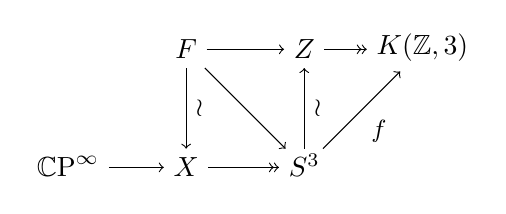
\begin{tikzpicture}[auto,node distance=1.5cm,
  main node/.style={font=\sffamily\bfseries},text height=1.5ex]
  \node[main node]   (S3) at (0,0)      {$S^3$};
  \node[main node]   (Z)  [above of=S3] {$Z$};
  \node[main node]   (K3) [right of=Z]  {$K(\Z,3)$};
  \node[main node]   (F)  [left  of=Z]  {$F$};
  \node[main node]   (X)  [left  of=S3] {$X$};
  \node              (K2) [left  of=X]  {$\cproj$};
  \path[every node/.style={font=\sffamily\small}]
    (F) edge [->] (Z)
    (F) edge [->] (S3)
    (F) edge [->] node [right] {$\wr$} (X)
    (S3) edge [->] node [right] {$\wr$} (Z)
    (Z) edge [->>] (K3)
    (K2) edge [->] (X)
    (X) edge [->>] (S3)
    (S3) edge [->] node [below right] {$f$} (K3);
\end{tikzpicture}
\end{center}

We now use the Serre Spectral Sequence of this last fibration. We know the homology groups of $S^3$ and $\cproj$, so we know the second page looks like this. Here the arrows are \emph{not} all isomorphisms.

\begin{center}
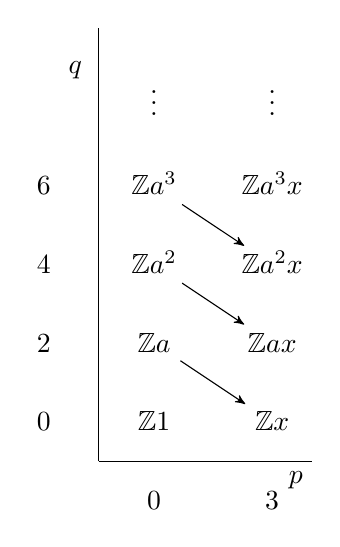
\begin{tikzpicture}[>=stealth',auto,node distance=1.5cm,
  text height=1.5ex]
  \node (00) at (0,0)      {$\Z 1$};
  \node (10) at (1.5,0)    {$\Z x$};
  \node (01) at (0,1)      {$\Z a$};
  \node (11) at (1.5,1)    {$\Z ax$};
  \node (02) at (0,2)      {$\Z a^2$};
  \node (12) at (1.5,2)    {$\Z a^2x$};
  \node (03) at (0,3)      {$\Z a^3$};
  \node (13) at (1.5,3)    {$\Z a^3x$};
  \node (04) at (0,4)      {$\vdots$};
  \node (14) at (1.5,4)    {$\vdots$};
  \node at (-1.4,0) {0};
  \node at (-1.4,1) {$2$};
  \node at (-1.4,2) {$4$};
  \node at (-1.4,3) {$6$};
  \node at (0,-1)   {0};
  \node at (1.5,-1) {$3$};
  \node at (1.8,-0.7)   {$p$};
  \node at (-1,4.5)   {$q$};
  \draw (-0.7,-0.5) -- (2,-0.5);
  \draw (-0.7,-0.5) -- (-0.7,5);
  \path[every node/.style={font=\sffamily\small}]
    (01) edge [->] (10)
    (02) edge [->] (11)
    (03) edge [->] (12);
\end{tikzpicture}
\end{center}
\end{example}

Since $X$ is 3-connected, $d:\Z a \to \Z x$ must be an iso, so we may assume $da=x$. Then $d(a^n)=na^{n-1}x$. Now we know what groups survive until $E_\infty$, to compute
\begin{align*}
H^i(X;\Z)&=\begin{cases} \Z_n & \text{if $i=2n+1$} \\ 0 & \text{if $i=2n$,} \end{cases} && \text{hence}&
H_i(X;\Z)&=\begin{cases} \Z_n & \text{if $i=2n>0$} \\ 0 & \text{if $i=2n-1$.} \end{cases}
\end{align*}
The Hurewicz Theorem modulo $\mc C$ now implies that the first $p$-torsion in $\pi_*(X)$, hence also in $\pi_*(S^3)$ is a $\Z_p$ in $\pi_{2p}$. For $p=2$ we get the stronger result that $\pi_4(S^3)=\Z^2$, hence also $\pi_{n+1}(S^n)=\Z_2$ for $n\geq3$.

\end{document}
